\chapter{Introdução} \label{ch:introdução}

A Internet é um conjunto de redes físicas heterogênea (uma variedade de dispositivos conectados, \textit{smartphones}, \textit{desktops}, \textit{notebooks}, servidores, \textit{switches}, roteadores, entre outros) funcionando como uma rede lógica única de alcance mundial. O grande e contínuo crescimento da Internet gerou um aumento da sua complexidade, que a expõe a diversas vulnerabilidades. 

A todo momento, novos ataques ou mesmo variações de ataques já existentes surgem e são lançados a várias redes indiscriminadamente em busca de vulnerabilidades. Em 2015, foram reportados ao Centro de Estudos, Respostas e Tratamento de Incidentes de Segurança no Brasil (CERT.br) cerca de 722.205 incidentes, em 2016, esse número diminuiu, chegando a 647.112 \cite{estatistica:cert.br}. Apesar da diminuição, esse número é considerado grande, presumindo-se que há muitos incidentes que não são reportados e/ou identificados.

As empresas, de qualquer segmento e tamanho, devem ter o trabalho de manter os ativos seguros e isso vai além da utilização de anti-vírus nos computadores. Ter uma política de atualização de \textit{software} em estações de trabalho e servidores, aliados com boas práticas nas configurações de serviços, dificultam a exploração de vulnerabilidades. 

A utilização de \textit{firewall}, não pode ser encarado com uma solução definitiva, passando uma falsa sensação de segurança, pois muitas portas legítimas podem estar vulneráveis, como acontece, por exemplo, com a porta 80 que hospeda \textit{websites} vulneráveis \cite{analisenessus:cleriston}.

Diante desse cenário, torna-se cada vez mais importante para o administrador de rede e/ou segurança da informação o uso de ferramentas de IDPS, permitindo identificar e tratar de forma automatizada os incidentes de segurança.

Para implementa tais ferramentas em uma rede, deve-se levar em consideração a flexibilidade e a administração simplificada para não resultar que a empresa/instituição fique na dependência de um único fabricante ou fornecedor da solução. Além disso, a ferramenta deve ter um bom desempenho e eficiência para não passar a falsa sensação de proteção ou degradar o desempenho da rede.

O CERT.br é o grupo de resposta a incidentes de segurança para a internet brasileira, mantido Comitê Gestor da Internet no Brasil. Atua na notificação e tratamento de incidentes de segurança dando apoio no processo de resposta. Além disso, faz um trabalho de conscientização e treinamento sobre problemas de segurança no Brasil. 

\begin{figure}[!htb]
 \centering
 \caption{Estatísticas de ataques reportadas ao CERT.br}
 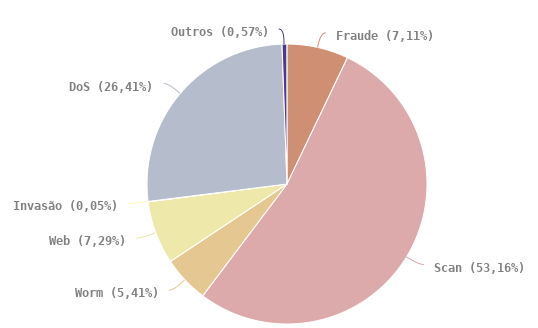
\includegraphics[scale=.6]{incidentes-reportados.png}
 \legend{Fonte: \cite{tipos-ataques:certs.br}}
 \label{fig:cert}
\end{figure}

Paralelamente ao CERT.br temos o Centro de Atendimento a Incidentes de Segurança (CAIS), mantido pela Rede Nacional de Ensino e Pesquisa (RNP). O CAIS é responsável por zela pela segurança da rede Ipê (infraestrutura de rede dedicada à comunidade brasileira de ensino superior), detectando, resolvendo e prevenindo incidentes de segurança. Além disso, tem o papel de orientar (através de publicações de cartilhas) e disseminar boas práticas de segurança da informação, educando e conscientizando usuários de todos os níveis sobre os principais riscos em segurança da informação \cite{cais}.

Desde 2008, todas a fraudes identificadas pelo CAIS estão sendo ordenadas e disponibilizadas para consulta (\autoref{fig:cais}). Adicionalmente, são enviados alertas através de uma lista quando uma fraude mostra-se particularmente perigosa aos usuários e computadores.

\begin{figure}[!htb]
 \centering
 \caption{Estatísticas de incidentes reportados ao CAIS}
 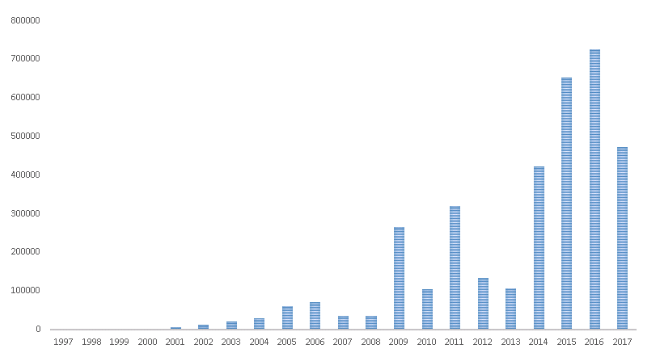
\includegraphics[scale=.7]{cais-incidentes-reportados.png}
 \legend{Fonte: \cite{cais}}
 \label{fig:cais}
\end{figure}

\section{Motivação} \label{sec:motivação} 

Escrever uma nova motivação

\section{Objetivos} \label{sec:objetivos}

Este trabalho tem como objetivo geral, avaliar e fazer um comparativo entre as soluções de código aberto de Sistemas de Detecção e Prevenção de Intrusão: Snort e Suricata. Como desdobramento de tal objetivo, os seguintes objetivos secundários foram definidos:

\begin{alineas}
\item Apresentar conceitos sobre segurança da informação e sua importância em um ambiente corporativo;
\item Descrever problemas relacionados a ataques envolvendo redes de computadores;
\item Descrever as ferramentas, compreendendo requisitos, características, modos de atuação e funcionalidades;
\item Descrever o ambiente experimental;
\item Realizar experimentos e coletar dados para validar o funcionamento e a eficiência das ferramentas;
\end{alineas}

\section{Metodologia} \label{sec:metodologia}

Esse trabalho se configura numa pesquisa qualitativa. Utilizou-se uma máquina com \textit{hardware} robusto, configurada com 130G de memória RAM, com um processador possuindo 40 núcleos e duas interfaces de rede, uma para gerência e outra configurada em modo '\textit{promisc}' com espelhamento do roteador. Nela instalou-se o SO XenServer versão 7, da Citrix, SO voltado para virtualização com um bom desempenho num ambiente de produção real. 

No \textit{host}, instalou-se duas máquinas virtuais, uma para cada ferramenta de IDPS em teste, Snort e Suricata, nas suas versões mais recentes, 2.9.8.3 e 4.0.0, respectivamente. A mesma quantidade de recurso de \textit{hardware} foi alocada para as máquinas, criando assim um ambiente igual para ambas as ferramentas. Além disso, após configuradas, usou-se a mesma base de assinaturas aberta da \textit{Emerging Threats} (ET), que possui frequentes atualizações.

As métricas para comparação avaliadas são a quantidade de recurso usado pela ferramenta para análise do tráfego em um período de tempo determinado, quantidade de falsos positivos e negativos e a taxa de detecção. Para avaliar os recursos de \textit{hardware}, usou-se dois recursos. Primeiro, foi instalado nas máquinas virtuais um \textit{daemon} collectd, a segunda forma, foi instalar um servidor de monitoramento Zabbix. 

Para facilitar a avaliação dos alertas gerados pelas ferramentas e determinar os falsos positivos e negativos, optou-se por centralizar o \textit{logs} em um servidor. Para tal, usou-se uma infraestrutura que reúne três serviços, descrito na \autoref{sec:infraestrutura}.

\section{Trabalhos Relacionados} \label{sec:trabalhos-relacionados}

O uso de ferramentas IDS \textit{opensource} Snort e/ou Suricata, importantes na área de segurança, já foi abordado e apresentou alguns resultados satisfatórios em pesquisas anteriores, por exemplo, nas pesquisas de Nagahama \textit{et al.} (2013), Martín \textit{et al.} (2014) e Cléber \textit{et al} (2014).

No trabalho do Nagahama \textit{et al.} (2013), é usado redes definidas por \textit{softwares}, que desacopla os planos de controle e de dados, permitindo adaptar o funcionamento da rede de acordo com a necessidade de cada um. O \textit{software} utilizado na pesquisa foi o OpenFLOW. Tal uso, tem como objetivo mitigar a falta de integração do IDS com os equipamentos de rede como {switches} e roteadores, o que limita a atuação destas ferramentas. 

Já Martín \textit{et al.} (2014), utiliza-se do BroFlow que possui uma série de vantagem, como, detecção de intrusão através de algoritmos simples, modular e flexível, reação imediata a um ataque descantando pacotes dos atacantes os mais próximo da origem. Dentre os resultados obtidos, destacam-se que a ferramenta conseguiu garantir o encaminhamento de pacotes legítimos na rede na taxa máxima do enlace e reduziu, em até dez vezes, o atraso na rede provocado pelo ataque.

No trabalho de Cléber \textit{et al} (2014), foi feito uma comparação de desempenho das ferramentas de IDS (Snort e Suricata) porém usou-se dados sintéticos fornecidos pela \textit{Defense Advanced Research Projects Agency} (DARPA) e devido ser uma base com ataques antigos, não houve resultados satisfatórios. Ao final, listou-se as vantagens e desvantagens existentes de cada ferramenta. No trabalho proposto, no entanto, serão usados dados mais próximo de um ambiente de produção. 

\section{Organização do Trabalho} \label{sec:organização-do-trabalho}

O restante desse trabalho está organizado da seguinte forma.

No \autoref{ch:segurança}, são definidos conceitos sobre redes de computadores e segurança da informação, também são descritos os ataques comuns e ferramentas utilizadas para validar e avaliar as soluções de IDPS.

Em seguida, no \autoref{ch:idps}, a definição IDPS, os tipos existentes, as funcionalidades e descrição das ferramentas avaliadas: Snort e Suricata.

O \autoref{ch:cenário-real} detalhará o cenário real e a infraestrutura utilizada para os realização dos testes das ferramentas, os testes realizados e o resultados obtidos.

Por fim, no \autoref{ch:considerações}, as considerações finais e trabalhos futuros.
